\subsection{Evaluaci\'on final del desempe\~no del software 2}
    La evaluaci\'on final del desempe\~no del software se centr\'o en
        medir el tiempo de simulaci\'on y la precisi\'on de las rutas
        generadas bajo diversas condiciones iniciales y sistemas
        operativos. Se comprob\'o que el algoritmo, aunque eficiente
        en la mayor\'ia de los casos, presenta diferencias de
        desempe\~no notables entre Windows y Linux, con mejores
        resultados en Linux debido a su mayor capacidad de
        procesamiento en simulaciones intensivas.
    \vskip 0.5cm
    %figura
    \begin{figure}[htbp]
        \centering
        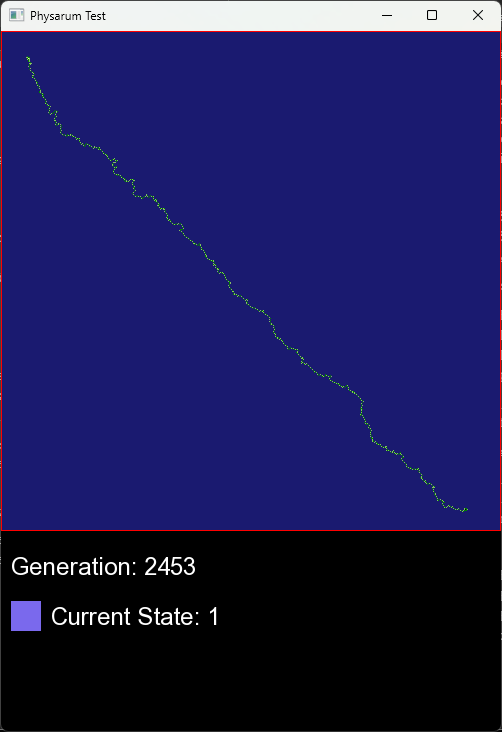
\includegraphics[width=0.5\textwidth]{./images/Pruebas/simulador/image085.png}
        \caption{Generaci\'on de una ruta despu\'es de el paso de generaciones en Windows (500 x 500)}
        \label{fig:Ruta 85}
    \end{figure}
    \vskip 0.5cm
    %figura
    \begin{figure}[htbp]
        \centering
        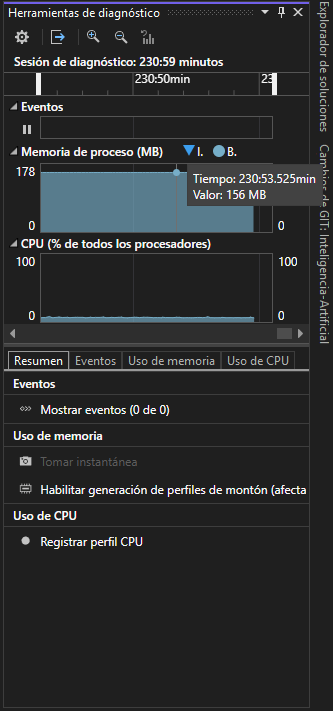
\includegraphics[width=0.5\textwidth]{./images/Pruebas/simulador/image086.png}
        \caption{Uso de la memoria y CPU durante la obtenci\'on de la ruta del Physarum.}
        \label{fig:Ruta 86}
    \end{figure}
    \vskip 0.5cm
    El an\'alisis de los tiempos de ejecuci\'on entre una generaci\'on
        y la siguiente permiti\'o identificar mejoras clave en la
        eficiencia del software. Los resultados mostraron que, en
        entornos de mayor complejidad, el tiempo de procesamiento
        incrementa proporcionalmente al n\'umero de barreras y
        obst\'aculos, lo que requiere optimizaciones adicionales en
        futuras iteraciones.